\chapter{Introduction}

Coronary atherosclerosis is a disease caused by the accumulation of material, mainly lipids and calcium, in the inner layer of the arterial wall, responsible for over 70\% of sudden cardiac deaths \cite{Czaja-Ziolkowska2022-pd}.
The buildup of calcium in the coronary arteries results in narrowing and hardening of the vessels affecting myocardial perfusion and increasing the risk for adverse cardiovascular events \cite{liu2015current}.
Calcified lesions develop for the action of multiple factors in a process that is not yet fully understood and for which a specific medical therapy, leading to reduction of calcium or at least limiting its progress, does not exist.
Coronary artery calcium (CAC) is a marker that reveals presence of atherosclerosis before its symptomatic phase.
CAC has been shown to be a good predictor for 10-year risk of cardiovascular disease (CVD) events such as coronary heart disease, myocardial infarction and strokes, regardless age, gender or ethnic group \cite{Budoff2018-uo} and its detection in the early development of atherosclerosis allows prompt intervention with therapies for reducing this risk.
For this reason CAC evaluation has become an important task of clinical screening.

CAC is usually estimated semi-quantitatively with a scoring method based on a semi-automatic procedure, that requires analysis of computed tomography (CT) scans by experts and can be time consuming and error prone.
CT is a non-invasive test that requires an expensive machine and exposes the patient to ionizing radiation; early detection of CAC would be improved if a reliable method for its evaluation could be found using a simpler and less dangerous screening test.
Trying to address to this need, the possibility of detecting CAC from chest X-ray (CXR) images using artificial intelligence (AI) is explored in this work.

In the last years, artificial intelligence and in particular deep learning (DL) techniques revolutionized many fields including computer vision, natural language processing and medical imaging.
This revolution became possible thanks to the continuous increase of the availability of data and  computational resources.
DL reached extraordinary results pairing human experts performance in analysis of medical images or even outperforming their human counterparts \cite{litjens2017survey} in some tasks like dermatology cancer detection \cite{esteva2017dermatologist} or diabetic retinopathy diagnosis \cite{gulshan2016development}.

The growing interest in CAC has led to many works \cite{vanvelzen2021ai} leveraging capabilities of AI for the automation of CAC evaluation.
This work use knowledge distillation (KD), an emerging DL techniques, aiming to use the knowledge learned by an artificial neural network trained on CT scans to drive CAC detection on CXRs.

In the following sections of this chapter the most widely used method for CAC scoring on CT scans will be described in details, then an overview of the medical images used for this work, CT scans and X-rays are presented, highlighting both their characteristics and differences.
Section \ref{sec:goal_of_this_work} is dedicated to explain the goal and contribute of this work, whereas related works are analyzed in section \ref{sec:related_works}.
The last section of this chapter will be an overview of the structure of this work.


\section{CAC score}

A CAC score is a numerical index used to estimate semi-quantitatively the amount of calcium in the coronary arteries\cite{Czaja-Ziolkowska2022-pd}.
Multiple methods can be used for calculating the CAC score, but the most widely employed in clinical practice is the Agatston method \cite{AGATSTON1990827}.
From now on, we refer exclusively to this method when talking of CAC score.

The Agatston method calculate CAC score from CT scan analysis using a semi-automated procedure.
After obtaining the CT scan, specialized software identifies high density regions, where the density is greater or equal to 130 Hounsfield units (HU), within each slice;
these regions are then reviewed by a medical expert to distinguish coronary calcifications from false positives, i.e. bones, implants, or calcifications that are not located within the coronary arteries.
For each confirmed area of coronary calcification, the software calculates an Agatston score by multiplying the area of the calcification by its corresponding density score.

The density score is determined based on the maximal density point of the area, in the following way:
\begin{itemize}
    \item 1 = 130 to 199 HU.
    \item  2 = 200 to 299 HU.
    \item 3 = 300 to 399 HU.
    \item 4 $\ge$ 400 HU. 
\end{itemize}
In the end, the final value is obtained by adding up each score of all selected areas.

The total Agatston score of a patient is correlated to a risk category of a 10-year CVD event according to table \ref{tab:agatston-risk}.
\begin{table}
    \centering
    \begin{tabular}{|c|c|}
        \hline
        Agatston score & Risk \\
        \hline
        0 & very low \\
        1-10 & low \\
        11-100 & intermediate \\
        101-400 & high \\
        > 400 & very high \\
        \hline
    \end{tabular}
    \caption{Risk categories based on Agatston scores \cite{vanvelzen2021ai}}
    \label{tab:agatston-risk}
\end{table}
It has been shown that a zero CAC score is associated with a low risk of CVD or death in both asymptomatic and even in symptomatic patients \cite{Czaja-Ziolkowska2022-pd} presenting chest pain or dyspnea.
On the contrary, even a minimal score below 10 on young people significantly increase possibility of coronary disease events, whereas values up to 100 on aged people can be considered less harmful, suggesting that CAC percentiles based on age (and also on gender) could be better predictors than CAC alone \cite{Czaja-Ziolkowska2022-pd} and also that its detection at young age, before symptoms, can be really important to prevent its development.

Calcium score can be calculated also on aortic and carotid arteries and on cardiac valves.
These scores cannot be used as CAC to estimate prognosis beyond other traditional risk factors \cite{Czaja-Ziolkowska2022-pd} like smoking, diabetes mellitus and family history of CVD, so they are not considered in this work; however they may have different applications, for example supporting diagnosis of stroke \cite{desai2018thoracic} or predicting outcome of transcatheter aortic valve implantation \cite{viegas2022significance}.
The possible presence of calcium lesions near the coronaries represent an additional complexity for the CAC detection task, that could result in a higher score due to false positives.


\section{CT scans and X-rays}

CT scans involve a computerized imaging technique where a rotating X-ray beam is directed through a patient; interactions of this beam with various tissues along its path are detected and processed to generate cross-sectional images of the patient's body, obtaining thus multiple slices which can be either analyzed individually or combined to create a 3D representation of the inner structures of the body.
Each pixel of the images represent the X-ray attenuation or the density of the tissue, its numerical value could depend on the scanner used but is usually converted using the Hounsfield scale.

Hounsfield scale assigns numerical values to each density using air and water as reference points. Air is assigned to -1000 HU, water to 0 HU.
Soft tissues of the body are usually around 0 HU whereas bones could be up to 1000 HU. Artery calcifications have density $\ge 130$ HU.
Usually values above bones density are considered noise, or could be metal prothesis, the same for values below air density, and then images are clipped to a min value of -1000 HU and a max value of 1000 HU.

Multiple CT protocols are commonly used for acquisition of images, depending on the specific exam the CT is performed for.
They may differ for some parameters that radiologists configure to achieve the better image for the task.
\begin{description}
    \item[Body part and zoom:] shall be chosen appropriately to be sure to visualize the interesting section with enough details.
    For calcium score CTs of the chest or of the cardiac area are required.
    \item[Radiations:] intensity of radiation emitted by the scanner is related to image quality, low-dose scans are preferred but produce noisy images.
    Low-dose chest CT scans, usually acquired for lung cancer screening, are not ideal for the task but some works have been done to try to use them for calcium scoring \cite{Lessmann_2018}.
    \item[Contrast enhancement:] scans could be enhanced using radiocontrast agents, in this case some structures of the body, like blood vessels, are more visible in the image, but their normal density is altered, calcium score is generally performed on non-contrast enhanced scans.
    \item[ECG-triggered:] to avoid motion artifacts of the heart the CT scanner could be synchronized with an ECG and images acquired only during specific phases of the cardiac cycle, this was usually required for calcium score, but became less important with advent of faster and better scanners.
    \item[Slice thickness and distance:] depending on the configuration and on the sensitivity of the scanner each image could represent a different slice thickness.
    Also slices could be contiguous, overlapping or with a certain distance between each other.
    Original protocol for calcium score requires 3mm thickness contiguous slices \cite{AGATSTON1990827}.
\end{description}

\begin{figure}
    \centering
    \begin{subfigure}[b]{0.3\textwidth}
        \resizebox{\textwidth}{!}{ 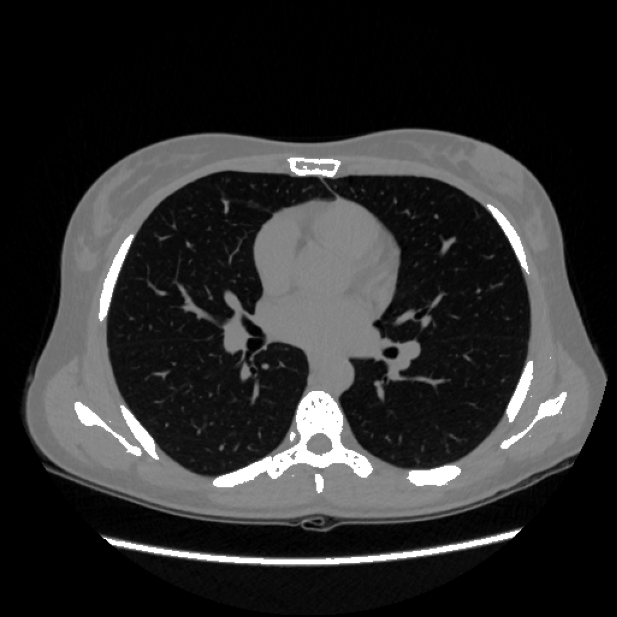
\includegraphics{ct_cac_0} }
        \caption{CAC = 0}
        \label{subfig:ct_cac_0}
    \end{subfigure}\hspace{1em}
    \begin{subfigure}[b]{0.3\textwidth}
        \resizebox{\textwidth}{!}{ 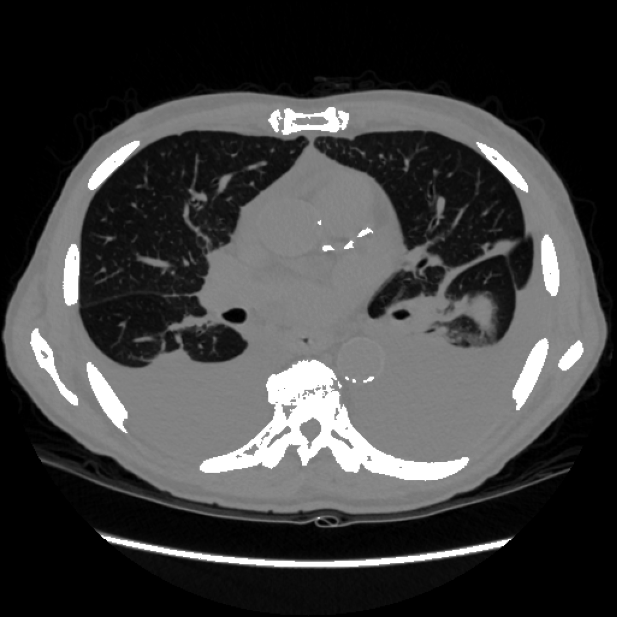
\includegraphics{ct_cac_1484} }
        \caption{CAC $\simeq$ 1500}
        \label{subfig:ct_cac_1500}
    \end{subfigure}\hspace{1em}
    \begin{subfigure}[b]{0.3\textwidth}
        \resizebox{\textwidth}{!}{ 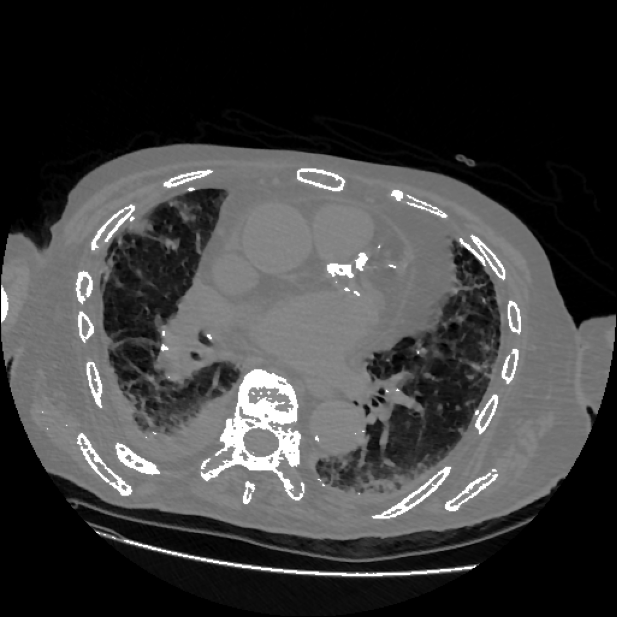
\includegraphics{ct_cac_4782} }
        \caption{CAC > 4000}
        \label{subfig:ct_cac_4000}
    \end{subfigure}
    
    \caption{Visualization of CT axial images with different values of CAC score. Calcium can be easily identified as the light areas near myocardium. Images from our dataset.}
    \label{fig:ct_cacs}
\end{figure}

CT scans are really well suited for CAC visualization.
As said, calcifications have a density above 130 HU, that is larger than density of every other tissue in the surrounding area, for this reason is simple to spot the lighter areas near myocardium.
From figure \ref{fig:ct_cacs} even an untrained eye can figure out a huge difference between an image without CAC \ref{subfig:ct_cac_0} and images with a large presence of calcium lesions.

Unfortunately, CT scans require expensive machines to capture images, are relatively slow and expose the patient to a not negligible amount of ionizing radiations.
This means they are not suitable for mass screening or routine testing, but shall be performed carefully, with proper evaluation of risks and benefits.

An older medical imaging procedure that is faster, cheaper and expose the patient to a smaller amount of radiations compared to CT scans is radiography, or commonly X-ray.
Radiographs are acquired using a device that emits a beam of X-rays towards the patient while on the other side of the patient a photografic film or a digital detector is placed to receive radiation passed through the body.
The result of this procedure is a single flat image of the inner of the body.
Just like CT scans, X-rays are based on tissue attenuation of radiation.
Dense tissues, like bones, are visualized as light areas in the image since they absorb an high amount of radiations, while soft tissues, allowing more radiations to pass through, are darker on the radiograph.

\begin{figure}
    \centering
    \begin{subfigure}[b]{0.4\textwidth}
        \resizebox{\textwidth}{!}{ 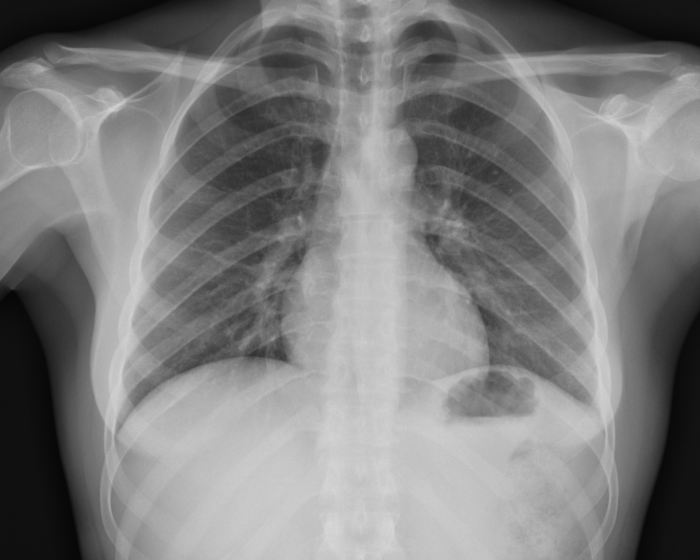
\includegraphics{cxr_cac_0} }
        \caption{CAC = 0}
        \label{subfig:cxr_cac_0}
    \end{subfigure}\hspace{1em}
    \begin{subfigure}[b]{0.4\textwidth}
        \resizebox{\textwidth}{!}{ 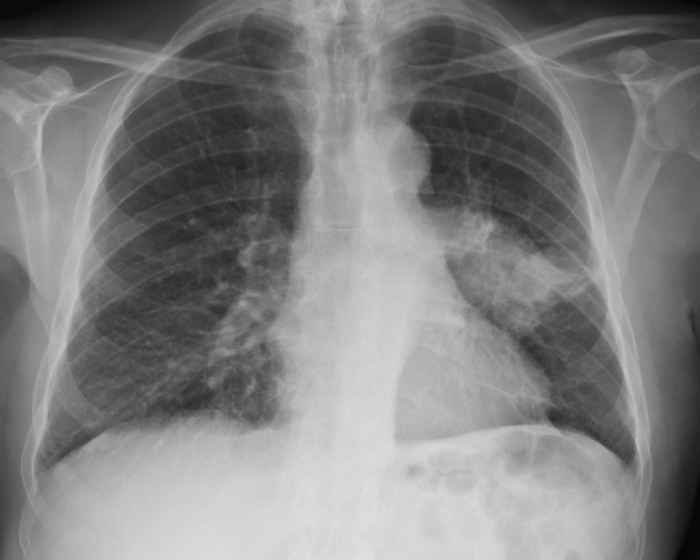
\includegraphics{cxr_cac_4947} }
        \caption{CAC > 4000}
        \label{subfig:cxr_cac_4000}
    \end{subfigure}
    
    \caption{Visualization of CXR images with different values of CAC score. Different amount of calcium cannot be clearly identified. Images from our dataset.}
    \label{fig:cxr_cacs}
\end{figure}

For CAC evaluation we use CXRs that are probably the most frequently-performed radiological investigation globally \cite{chest_radiograph}.

CXRs can be performed in different projections based on where the X-ray emitter and detector are placed in relation to the patient.
The three main projections used for CXR are:
\begin{enumerate}
    \item \textbf{PA:} posteroanterior view, the standard projection performed when emitter is placed behind the patient. It is considered the best projection to visualize lungs, heart and great vessels \cite{chest_radiograph}
    \item \textbf{AP:} anteroposterior view, when emitter is placed in front of the patient. It is required when the patient is not able to stand for a PA, can be performed even on patients lying in bed or using mobile X-ray devices. The quality of produced images is lower and the heart appears bigger due to its distance to the detector
    \item \textbf{Lateral:} lateral view, emitter and detector are placed on the side of the patient. Usually performed in conjunction with a PA
\end{enumerate}

Compared to CT scans, quality of images produced by X-rays is lower and since it is a 2D projection some details might be hidden by other parts of the body.
They are often used as a first diagnostic exam to determine if further analysis are required or not.
From figure \ref{fig:cxr_cacs} is possible to see that different amount of CAC cannot be easily discerned from CXR images.


\section{Goal of this work}\label{sec:goal_of_this_work}
The aim of this thesis work is to investigate the possibility to detect on CXRs the presence of coronary calcifications using neural networks (NN).
This is considered an hard task even for expert radiologists since CXRs are not as detailed as CT scans and also calcium lesions could be partially hidden by chest bones in radiographs.

The NN shall be built to solve a binary classification problem, i.e. to split the set of patients in two classes, using only CXR images as input.
Each patient is assigned to a class based on its CAC score:
\begin{itemize}
    \item \textbf{POSITIVE:} CAC > 0
    \item \textbf{NEGATIVE:} CAC = 0
\end{itemize}

For our purposes, a specific dataset has been constructed by \emph{Città della Salute e della Scienza di Torino} hospital; the latter is composed of 603 patients.
For most of the patients we have both a CT scan and a frontal CXR available, performed within a short period of time from each other.
All patients are labeled by an expert with the CAC score.

The work is composed by two main parts:
\begin{enumerate}
    \item Training of a NN on CTs that is able to classify patients in the two defined classes
    \item Distillation of knowledge learned by the network trained at step 1 to a NN working on CXRs
\end{enumerate}


\section{Related works}\label{sec:related_works}
Thanks to recent discoveries in the field of artificial intelligence, many calcium scoring methods which exploit machine learning have been proposed in last years \cite{vanvelzen2021ai}.
Most of these methods are based on analysis of CT scans, following the same procedure performed by experts, namely extract lesion candidates based on density (usually $\ge$ 130HU), identify real calcifications in the area of interest, and finally calculate Agatston score; automatic CAC scoring aims to replace the second step using a classifier.

\citeauthor{Wolterink2015-ii} \cite{Wolterink2015-ii} proposed a method that first extracts relevant features, (i.e. size, shape, intensity and location) out of each lesion candidate, and then applies classifiers composed by an ensemble of randomized decision trees to determine if it is a coronary calcification and also on which of the three major coronary arteries it is placed.
Classification errors are also mitigated presenting uncertain results to an expert for potential correction.

Some works aim to extract CAC score out of CT scans performed for various analysis, and then not optimized specifically for this task: \citeauthor{Lessmann_2018} \cite{Lessmann_2018} for example used low-dose CT scans performed for lung cancer screening to extract also CAC score information.
They proposed to use two convolutional neural network (CNN) in serie: the first used dilated convolutions to develop a large receptive field allowing to evaluate if the lesion candidate position is compatible with expected, the second exploited a small receptive field to classify the candidate based on local information.
Their method achieved a 90\% accuracy in classification into risk categories compared to manual annotation.

\citeauthor{Cano-Espinosa2018-gm} \cite{Cano-Espinosa2018-gm} and \citeauthor{de_Vos_2019} \cite{de_Vos_2019} embraced a different approach, directly regressing CAC score using CNNs.
\citeauthor{Cano-Espinosa2018-gm} achieved 75.6\% correct risk category classification using non-ECG gated CT scans: this might seem a poor result, but on these kind of CTs many artifacts due to heart motion that can alter appearance of coronary calcifications are present.
\citeauthor{de_Vos_2019} \cite{de_Vos_2019} achieved a minimum of 93\% on risk category classification using CTs captured with different protocols, they also improve their method providing a feedback heat-map showing on the image the pixels that contribute the most to the score, solving a common concern on direct application of NN as a black box to solve the CAC score task.

Most of the works available in literature and all those cited so far used CT scans to perform CAC classification or regression.
Possibility to use CXRs for CAC evaluation has been preliminary explored in a very limited number of works, only two on our knowledge:
\citeauthor{kamel_2021} \cite{kamel_2021} used a VGG-16 \cite{simonyan2015deep} deep CNN pre-trained on ImageNet dataset \cite{imagenet_cvpr09} to discern zero CAC patients from non-zero CAC, they also adapted the network to detect CAC per coronary artery and to detect CAC above and below a fixed threshold.
They used a dataset of 1689 radiographs and achieved an accuracy of 71\% on a test set of 231 images for the zero/non-zero task.

Furthermore, in \cite{iodice_2022} the author used the same dataset available for this work to discern low risk patients with CAC < 10 from higher risk patients.
He exploited a DenseNet-121 \cite{huang2018densely} pre-trained on CheXpert dataset \cite{Irvin_2019} replacing the final classifier with 2 fully-connected layers.
The results are an average accuracy of 79\% and a balanced accuracy (BA) of 77\% measured using 5-fold cross validation.

Aiming to resolve a completely different task, but using a similar approach of that proposed in this work, \citeauthor{zhang2023distilling} \cite{zhang2023distilling} used multi-modal knowledge distillation to detect endometriosis: they trained a teacher model on ultrasound video clips, then distilled its knowledge to a student model that works on magnetic resonance images which is a modality where endometriosis is considered harder to detect.
They have been able to improve performance of the model starting from an area under curve (AUC) of 65\% using a naive approach, to 90.6\% using pre-training and knowledge distillation.


\section{Overview of the thesis}
This thesis work is composed of six chapters.
After this introduction, a summary of deep learning and main concepts applied to develop the work is presented in chapter \ref{sec:deep_learning}.
A particular focus is dedicated to describe knowledge distillation and transfer learning, the two techniques we used to improve training performance.
\\
On chapter \ref{sec:dataset}, we describe the dataset used to train our models, analysing data distribution and discussing potential biases.
\\
On chapter \ref{sec:method} we show step by step the method developed to train a NN for CAC classification using CXR images, including image pre-processing details, the network architectures chosen, and the training procedure and parameters.
This chapter is composed of two main sections: the first describes what we did to train some models on CT scans, the second explains how we performed training on CXRs, our implementation of knowledge distillation and how we created reference models to evaluate results.
\\
After describing the applied method, in chapter \ref{sec:experiments} we analyze the results of the many experiments performed, comparing the performance of our method with the state of the art.
We started experimenting with a single modality of our data at a time, i.e. only CT scans and only CXRs, to create the basic models to use as reference and for KD, then we compared two different approaches of KD and also KD mixed with transfer learning.
\\
Finally, in chapter \ref{sec:conclusion} we present our conclusions and possible improvements.
